%
% File ccl2024-zh.tex
%
%%
%% Based on the original version of COLING-2018 file (coling2018.tex), with changes made by Yue Zhang.
%%

\documentclass[11pt]{article}
\usepackage{ctex}
\usepackage[utf8]{inputenc}
\usepackage[hyperref]{ccl2024-zh}
\usepackage{url}
\usepackage{latexsym}
\usepackage{CJKutf8}
\usepackage{indentfirst}
\usepackage{fancyhdr}
\usepackage{graphicx}
\usepackage{tabularx}

\pagestyle{fancy}
\fancyhf{}
\lhead{\begin{CJK*}{UTF8}{gbsn}计算语言学\end{CJK*}}
\renewcommand{\headrulewidth}{0pt}

% \setlength\titlebox{5cm}

% You can expand the titlebox if you need extra space
% to show all the authors. Please do not make the titlebox
% smaller than 5cm (the original size); we will check this
% in the camera-ready version and ask you to change it back.



\title{基于CQL的语料库检索引擎设计}
\englishtitle{Design of corpus retrieval engine based on CQL}

\date{}


\begin{document}
\begin{CJK*}{UTF8}{gbsn}
\setlength{\parindent}{2em}

% Make Chinese title and abstract
\maketitle
\begin{abstract}
  这是摘要。
  \keywords{CQL \and 语料库}
\end{abstract}

% Make English title and abstract
\makeenglishtitle
\begin{englishabstract}
  This document.
  
  \englishkeywords{First keyword \and Second keyword}
\end{englishabstract}


\section{引言}
\label{intro}

%
% The following footnote without marker is needed for the camera-ready
% version of the paper.
% Comment out the instructions (first text) and uncomment the 8 lines
% under "final paper".
%
\cclfootnote{
    %
    % for review submission
    %
    \hspace{-0.65cm}  % space normally used by the marker
    % 最终版论文请将许可声明放在此处。请参阅说明中的~\ref{licence}部分来准备论文。
    \textcopyright 2024 中国计算语言学大会

    \noindent 根据《Creative Commons Attribution 4.0 International License》许可出版
}

\section{背景}
\label{backgound}

在计算语言学的研究领域中,语料库检索工具扮演着至关重要的角色。对于自然语言工作者而言,如何高效、准确地从庞大的语料库中检索到所需信息,是他们日常工作中必须面对的挑战。然而,目前语料库检索表达式的非通用性成为了制约其广泛应用的一大瓶颈。

语料库检索的复杂性和多样性主要体现在其检索表达式的非标准化上。例如,北京大学现代汉语语料库、北京语言大学BCC语料库等中文语料库,虽然各自拥有庞大的语料资源,但它们的检索表达式却互不兼容。这意味着用户在使用这些语料库时,需要分别学习和掌握各自的检索语法和规则,这无疑增加了学习成本和使用难度。

CQL(Corpus Query Language)作为一种语法简单、易于掌握的语料库检索语言,得到了广泛的应用。然而,目前支持CQL的中文语料库还相对较少,这使得CQL的应用受到了一定程度的限制。

随着人工智能技术的快速发展,大语言模型为语料库检索带来了新的机遇。大语言模型通过深度学习和自然语言处理技术,能够实现对语义向量的理解和自然语言的处理,从而改进检索效率和质量。

设计一款能够支持CQL语言检索、语义检索、自然语言检索的语料库检索服务,对于减轻用户学习负担、提高检索效率和质量具有重要意义。

\subsection{CQL语言}

随着信息技术的飞速发展,语料库作为语言学研究的重要工具,其查询语言也经历了不断的演变与完善。其中,语料库查询语言(Corpus Query Language,简称CQL)作为从CQP(Corpus Query Processor)发展而来的一系列语言,已经逐渐成为语料库检索领域的主流语言。CQLF(Corpus Query Lingua Franca)已经成为国际标准ISO 24631-1(ISO 2018),在国际范围内的广泛认可与应用。

目前,众多语料库检索工具均采用了CQL作为检索语言,如CQPweb、Sketch Engine、BlackLab等。这些工具使用CQL为用户提供高效、便捷的语料库检索体验。具体来说,CQL语言包括以下几个关键元素:

(1)检索单元:检索单元是由基本检索式以及逻辑运算符构成的,用于指定检索的标签以及具体的检索值。其中检索标签是在语料库设计时预先定义的,例如:word、lemmon、pos等。检索值即具体的查询内容,可以是词语、词性等内容。此外,CQL还支持使用正则表达式进行词语的匹配。基本检索式可以通过布尔运算符进行连接,组成复合检索式。

(2)单元数量约束:在CQL中,一个检索语句可以由多个检索单元组成。在进行语料匹配时,检索系统会对检索内容从左到右进行检索单元的匹配,每个检索单元可以通过{m,n}的形式指定其重复次数,实现对检索结果的控制。

(3)检索范围操作符:为了进一步提高检索的灵活性,CQL还提供了within操作符,用于限定检索范围。这使得用户可以在特定的文本片段进行检索。

(4)全局限定标签:CQL还支持全局限定标签的使用,这使得用户可以在对检索单元赋予一个标签名,然后通过"::"后面的全局限定条件,通过标签之间的逻辑关系,对检索单元进行约束。

\subsection{倒排索引}

在语料库设计中,需要根据语料库系统采用的标签,建立这些标签和文档之间的倒排索引信息。

倒排索引是一种记录关键词出现在文档中的方式,通过记录关键词出现在那些文档的方式,建立关键词到文档的索引关系,从而提高搜索效率和匹配度。

语料库检索可以看作是通过标签信息检索到包含这些标签的文档的过程。语料库中一些常用的标签包括:词语、词性、词长等信息,这些都可以作为关键字建立标签与文档之间的倒排索引。

倒排索引技术,作为一种高效的信息检索手段,在现代信息处理和搜索引擎中发挥着关键作用。它的核心思想是根据文档内容生成一个索引,这个索引以单词或短语等关键元素为索引项,将文档中出现这些元素的位置信息或文档标识与之关联。通过这种方式,当用户输入查询请求时,系统能够迅速定位到包含相关元素的文档,从而极大地提高了检索速度和准确性。

具体来说,倒排索引的构建过程通常包括分词、统计词频、建立索引表等步骤。分词是将文本拆分成单词或短语的过程,而统计词频则是为了确定每个词在文档中的重要性。随后,系统会根据这些信息建立一个索引表,其中包含了单词或短语到文档位置的映射关系。

在检索过程中,用户输入的查询请求会被系统解析成关键词,然后系统会在倒排索引中查找这些关键词对应的文档位置信息。由于倒排索引已经预先建立了关键词与文档之间的关联,因此系统能够迅速找到相关的文档,并按照一定的排序规则(如相关性、时间等)返回给用户。

倒排索引技术的优点在于其高效性和灵活性。通过预先建立索引,系统能够在短时间内处理大量的查询请求,同时支持复杂的查询操作和个性化的排序方式。此外,倒排索引还可以方便地支持增量更新和扩展,以适应不断变化的文档集合和查询需求。

然而,倒排索引技术也面临一些挑战和限制。倒排索引对于语义信息的处理相对较弱,难以处理一些复杂的查询需求,如语义相似度匹配等。

\subsection{语义检索}

语义搜索是指搜索引擎的工作不再拘泥于用户所输入请求语句的字面本身,而是透过现象看本质,准确地捕捉到用户所输入语句后面的真正意图,并以此来进行搜索,从而更准确地向用户返回最符合其需求的搜索结果。

语义向量检索是一种基于深度学习和自然语言处理技术的信息检索方法,旨在更准确地捕捉和理解文本中的语义信息,以实现更高效、更精准的检索结果。与传统的基于关键词匹配的检索方法不同,语义向量检索通过将文本转化为高维的向量表示,能够捕捉文本间的深层语义关系,从而更好地满足用户的查询需求。

在语义向量检索中,首先需要通过训练深度学习模型,如词嵌入模型或句子嵌入模型,将文本转化为向量表示。这些向量不仅包含了文本的表面信息,还融入了语义、上下文等深层信息,使得相似的文本在向量空间中更加接近。

当用户输入查询请求时,系统会将查询文本转化为语义向量,并在预先构建的向量索引中查找与之相似的向量。这些相似的向量代表了与查询文本具有相似语义的文档或信息。系统可以根据向量的相似度得分对结果进行排序,并返回给用户。

\section{我们的工作}

我们经过深入研究和对比,最终选择了CQL语言作为我们的语料库检索语言。这一选择旨在统一并简化检索语法,提升用户的使用体验。基于这一决策,我们设计并开发了一款功能强大的语料库检索引擎,该引擎支持CQL语言检索、语义向量检索以及自然语言检索,为用户提供了多元化的检索途径。

在实现过程中,我们采用了ANTLR工具进行CQL语言的解析,确保了语法解析的准确性和高效性。同时,我们利用倒排索引技术建立了语料数据库,有效提升了检索速度和准确性。为了支持语义向量检索,我们结合了BGE与FAISS的强大功能,实现了高精度的语义匹配。

我们还借助先进的大语言模型技术,实现了自然语言到CQL的转换功能。这一创新性的设计使得用户能够使用自然语言进行检索,无需掌握复杂的CQL语法,极大地降低了学习成本,提升了检索的便捷性。

\subsection{CQL语法解析}

CQL具有良好的人类可读性,但如果使用CQL实现语料库的检索,还需要将其转换为计算机可执行的结构化查询语句。
实现语法解析可以采用语法分析工具,ANTLR是一款强大的开源语法分析工具,使得开发一门新语言的工作转变为使用扩展巴斯科范式(Extended Backus–Naur Form,简称 EBNF)来描述语法。极大的简化了语言的解析工作。CQL符合EBNF定义,因此可以将CQL转换为EBNF语法文件。通过ANTLR工具,可以为CQL语法文件,生成相应的词法/语法分析器。
在\footnote[1]{https://github.com/exquery/corpusql-parser}提供的CQL语言描述文件的基础上,使用ANTLR工具生成了Python3版本的语法解析器。用户可以利用语法解析器将输入的CQL文本转换成语法树,语法解析器提供了Listener接口,可以通过该接口遍历语法树。
以“[word='把'|word='被'][]{0,10}[word='给']WITHIN <s>”为例,通过遍历,生成的语法树结构如图所示:

\begin{figure}[h]
	\centering
	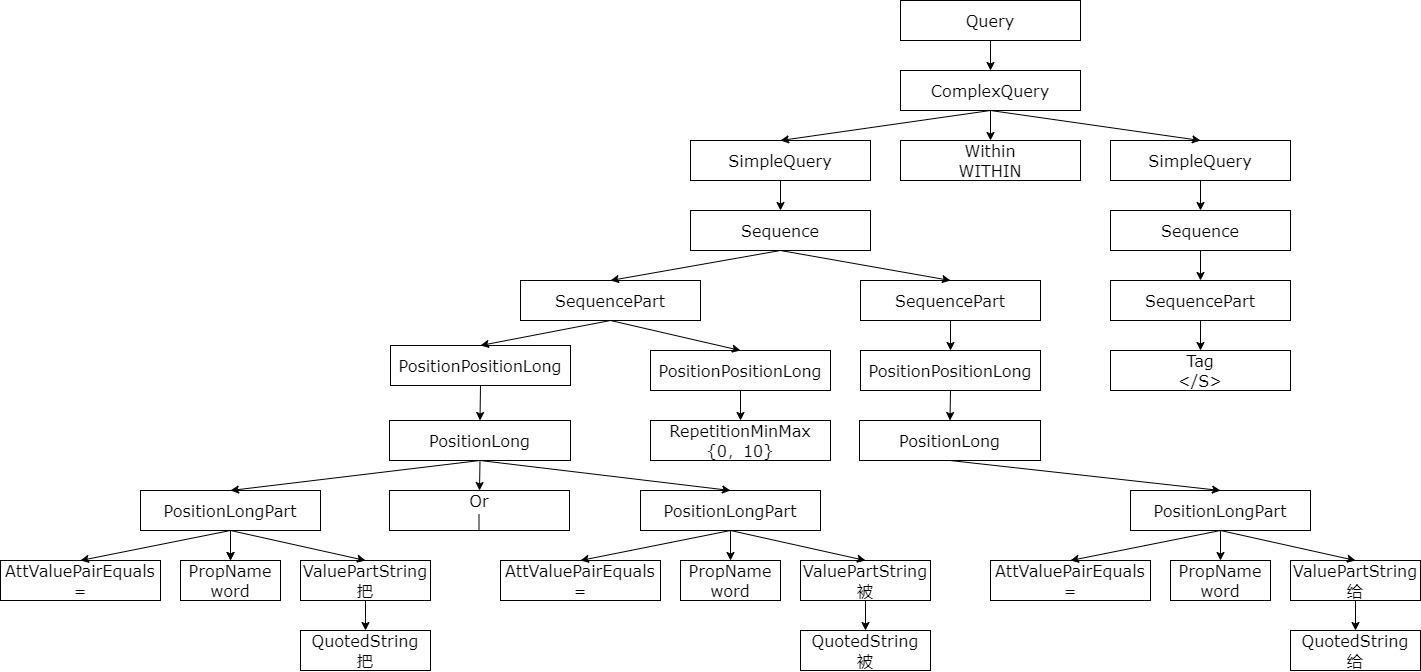
\includegraphics[width=0.7\textwidth]{cql-tree.jpg}
	\caption{CQL语法树}
	\label{fig:example}
\end{figure}

\subsection{倒排索引表设计}

检索和核心任务是完成检索词到文档的匹配,原始文本经过统一编码,段落分割、句子分割等预处理后,形成统一格式的语料数据。倒排索引工具,首先将传入的语料数据进行分段、分句操作,然后让每一句话通过分词工具进行分词以及标注词性,统计词频和词长等信息,建立倒排索引表。

文档包含的信息是具有层次结构的,一篇文档,有很多属性信息包括:作者、文件名称、文件类型、文件大小、创建时间等信息,文件的内容还可以分为多个段落,每个段落由多个句子构成,在建立倒排索引是充分考虑文章的属性信息以及结构信息,建立具有层级关系的倒排索引。

倒排索引的标签范围不仅是词语、还可以是词性、词语原型等任何可标签化的信息。并且倒排索引索引到的内容不是文档ID,而是索引到句子ID。

\begin{figure}[h]
	\centering
	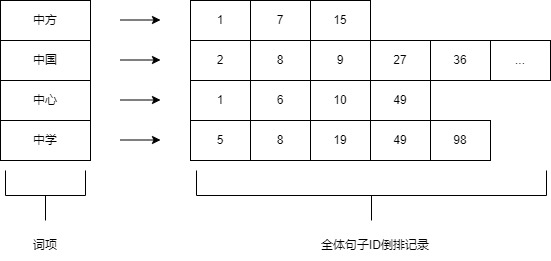
\includegraphics[width=0.6\textwidth]{r-index.jpg}
	\caption{倒排索引表}
	\label{fig:example}
\end{figure}

将用户输入的检索语句,分割出检索单元,通过遍历方式对检索树中的检索单元执行检索,返回与检索树匹配的所有可能句子或段落,这时匹配的候选结果仅能保证符合当前检索单元的匹配要求。

采用两阶段检索策略,第一阶段搜索语料库,仅作检索片段的匹配,忽略检索片段的位置和距离约束,找到所有可能的匹配文档, 第二阶段对每个文档进行位置和距离约束匹配。筛选出满足约束的文档作为候选。

依次遍历检索式中的所有检索单元,将所有检索单元的结果做布尔运算,得到了待选列表。然后对待选列表中每一项,与检索单元进行匹配,依次找出所有可能的匹配节点,通过动态规划算法验证这一项符合检索式要求,然后将这一项加入到候选列表中。

\subsection{两阶段检索策略}

检索和核心任务是完成检索词到文档的匹配,原始文本经过统一编码,段落分割、句子分割等预处理后,形成统一格式的语料数据。倒排索引工具,首先将传入的语料数据进行分段、分句操作,然后让每一句话通过分词工具进行分词以及词性标注,统计词频和词长等信息,建立倒排索引表。

文档包含的信息是具有层次结构的,一篇文档,有很多属性信息包括:作者、文件名称、文件类型、文件大小、创建时间等信息,文件的内容还可以分为多个段落,每个段落由多个句子构成,在建立倒排索引是充分考虑文章的属性信息以及结构信息,建立具有层级关系的倒排索引。

倒排索引的标签范围不仅是词语、还可以是词性、词语原型等任何可标签化的信息。并且倒排索引索引到的内容不仅是文档ID,还包括索引到句子ID、段落ID等具体的检索单元。


将用户输入的检索语句,分割出检索单元,通过遍历方式对检索树中的检索单元执行检索操作,返回与检索树匹配的所有可能句子或段落,这时匹配的候选结果仅能保证符合当前检索单元的匹配要求。

采用两阶段检索策略,第一阶段搜索语料库,仅作检索片段的匹配,忽略检索片段的位置和距离约束,找到所有可能的匹配文档, 第二阶段对每个文档进行位置和距离约束匹配。筛选出满足约束的文档作为候选。

\subsection{检索单元查询}

简单检索式可以在直接对应语料库的一次查询动作,根据用户输入的标记,以及指定的检索范围进行倒排索引的匹配,找到复合检索条件的文档ID。
复合检索式经过语法解析后,生成由简单检索式和逻辑运算符组成的二叉检索树,通过遍历检索树并对每个简单检索式的检索结果按照逻辑运算符进行逻辑运算,即可返回复合检索式的检索结果。

\begin{figure}[h]
	\centering
	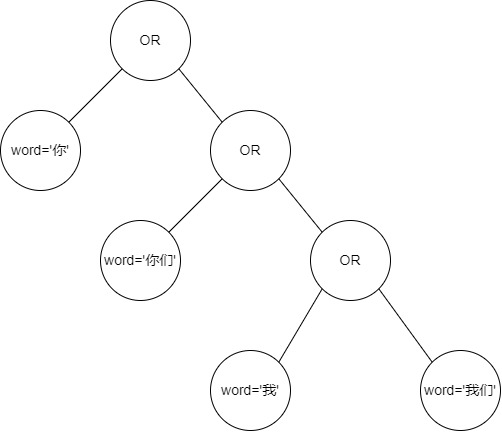
\includegraphics[width=0.5\textwidth]{node-tree.jpg}
	\caption{搜索树}
\end{figure}


\subsection{复合语句查询}

依次遍历检索语句中的所有检索单元,将所有检索单元的结果做布尔运算,得到了待选列表。然后对待选列表中每一项,与检索单元进行匹配,依次找出所有可能的匹配节点,通过动态规划算法验证这一项符合检索式要求,然后将这一项加入到候选列表中。

\begin{figure}[h]
	\centering
	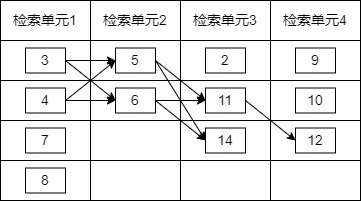
\includegraphics[width=0.5\textwidth]{dy.jpg}
	\caption{搜索树}
\end{figure}
非连续词语检索

\subsection{全局匹配条件}

语言成分边界标记其一般形式为:WITHIN x 或者 x CONTAINING ,x是语言成为标记,可以是:\textless s \textgreater 句子边界、\textless u \textgreater 话轮边界等,起到限定检索范围,防止跨语言边界检索的目的。

本文定义了\textless s \textgreater、\textless p \textgreater 、\textless t \textgreater 三种检索边界标记,可以指定检索范围是句子,或者是段落、或者是文档。
在实现式,通过建立句子、和段落级别的倒排索引,实现对检索边界标记的支持,默认的检索范围为段落。


\subsection{语义向量查询}

语义向量模型作为语言模型的核心组成部分,在文本处理和信息检索领域扮演着举足轻重的角色。这一模型通过将文本转换为高维向量表示,突破了传统文本字符的限制,使得我们可以在语义层面上进行精确匹配和相似性计算。本文深入研究了语义向量模型在文档检索中的应用,并采用了智源的bge-base-zh-v1.5模型作为我们的主要工具。这一模型具有强大的语言处理能力,支持长达512长度的输入文本,为我们在不同文本长度上进行向量表示提供了可能。

在用户进行文档检索时,其需求可能涉及句子、段落或整个文档等不同层次的信息。因此,在构建语义向量索引时,我们采用了分级策略,即按照句子、段落和文档三个层级建立相应的语义向量索引。这种分级索引不仅提高了检索的精度,也增强了检索的灵活性,使得用户可以根据自己的需求在不同层次上进行检索。

然而,由于BGE语义向量模型所支持的最大token长度为512,我们在处理较长的文本时,需要采用滑动窗口方法。这种方法可以在文本块之间保留一定的重叠,确保语义上下文在文本块之间不会丢失,从而保证了生成的语义向量的准确性和完整性。通过这种方法,我们成功地为文本生成了768维的语义向量,这些向量能够精确地表示文本的语义信息。

在语义向量的保存与检索方面,我们采用了FaceBook的AI团队开发的Faiss(Facebook AI Similarity Search)检索库。这一工具为我们提供了高效的向量数据库建立和检索功能。我们利用Faiss的IndexIVFFlat索引方式,将生成的语义向量存储到向量数据库中,并通过欧氏距离来计算向量之间的相似度。这种相似度计算方式能够准确地反映向量之间的语义关系,为我们在文档检索中提供了有力的支持。

综上所述,通过采用智源的bge-base-zh-v1.5模型、滑动窗口方法以及Faiss检索库,我们成功地构建了基于语义向量的文档检索系统。这一系统能够在语义层面上进行精确匹配和相似性计算,为用户提供了更加高效、准确的文档检索体验。

\subsection{自然语言查询}

在本文中,我们参考了《从文本到 CQL:连接自然语言和语料库搜索引擎》这篇论文,利用大语言模型实现了自然语言到语料库检索语言(CQL)的转换,从而实现了使用自然语言进行语料库检索的目标。大语言模型具有强大的语言理解和生成能力,能够准确捕捉用户输入的语义信息,并将其转化为符合CQL规范的查询语句。通过这种方法,用户可以更加直观地表达自己的检索需求,无需了解复杂的CQL语法规则,提高了检索的便捷性和效率。实验结果表明,我们的大语言模型在转换自然语言到CQL方面取得了显著的效果,为语料库检索领域带来了新的突破。

\section{实验}

\subsection{数据集}


\subsection{检索式对比}

CCL语料库检索式设计十分完善。然而,对于初学者而言,其学习成本相对较高。具体而言,CCL查询表达式中定义了多达13个特殊符号,其检索式由基本项、简单项、复杂项、过滤项、子句等多个部分组成,这就要求使用者必须掌握这些基础知识才能有效地编写检索表达式。

相比之下,CQL语言在语法上显得更为简洁直观。通过使用CQL表达式,用户能够更快速地掌握语料库的使用方法,无需投入过多的时间和精力去学习和记忆复杂的符号和规则。通过对比一些常用的检索式写法,我们可以清晰地看到CQL的简洁性。相较于CCL中使用的特殊符号和复杂的结构,CQL提供了一种更为直接和自然的方式来表达检索需求,从而提高了检索的效率和用户体验。


\begin{table}[h]
	\begin{center}
		\begin{tabular}{|c|c|c|}
			\hline \bf CCL检索式 & \bf CQL检索式 & \bf 说明 \\ \hline
			被+1把+6给 & word='被'][]{1}[word='把']{6}[word='给'] & 查出同时含有“被”“把”“给”的句子。 \\
			被+1把+6给 & word='被'][]{1}[word='把']{6}[word='给'] & 查出同时含有“被”“把”“给”的句子。 \\
			被+1把+6给 & word='被'][]{1}[word='把']{6}[word='给'] & 查出同时含有“被”“把”“给”的句子。 \\
			被+1把+6给 & word='被'][]{1}[word='把']{6}[word='给'] & 查出同时含有“被”“把”“给”的句子。 \\
			\hline
		\end{tabular}
	\end{center}
	\caption{\label{font-table} CQL与CCL检索式对比}
\end{table}

通过对比可以看到,CCL检索式和CQL检索式能够实现的功能基本相同,但CQL检索式的形式和规则比较简单,采用统一的约束符号,更容易被掌握。

\subsection{检索质量实验}

检索质量

\subsection{检索速度实验}

检索速度

\section{结论}

结论


% include your own bib file like this:
%\bibliographystyle{ccl}
%\bibliography{ccl2022-zh}

\begin{thebibliography}{}

\bibitem[\protect\citename{Aho and Ullman}1972]{Aho:72}
Alfred~V. Aho and Jeffrey~D. Ullman.
\newblock 1972.
\newblock {\em The Theory of Parsing, Translation and Compiling}, volume~1.
\newblock Prentice-{Hall}, Englewood Cliffs, NJ.

\bibitem[\protect\citename{{American Psychological Association}}1983]{APA:83}
{American Psychological Association}.
\newblock 1983.
\newblock {\em Publications Manual}.
\newblock American Psychological Association, Washington, DC.

\bibitem[\protect\citename{{Association for Computing Machinery}}1983]{ACM:83}
{Association for Computing Machinery}.
\newblock 1983.
\newblock {\em Computing Reviews}, 24(11):503--512.

\bibitem[\protect\citename{Chandra \bgroup et al.\egroup }1981]{Chandra:81}
Ashok~K. Chandra, Dexter~C. Kozen, and Larry~J. Stockmeyer.
\newblock 1981.
\newblock Alternation.
\newblock {\em Journal of the Association for Computing Machinery},
  28(1):114--133.

\bibitem[\protect\citename{Gusfield}1997]{Gusfield:97}
Dan Gusfield.
\newblock 1997.
\newblock {\em Algorithms on Strings, Trees and Sequences}.
\newblock Cambridge University Press, Cambridge, UK.

\end{thebibliography}

\end{CJK*}
\end{document}

